\documentclass[journal]{IEEEtran}
\usepackage[T1]{fontenc}
\usepackage{cite}
\usepackage{amsmath,amssymb}
\usepackage{booktabs,array,tabularx,multirow}
\usepackage{graphicx}
\usepackage{xcolor}
\usepackage{tikz}
\usetikzlibrary{positioning,arrows.meta,calc}
\usepackage[hidelinks]{hyperref}
\makeatletter
\setlength{\@fptop}{0pt}
\setlength{\@fpsep}{16pt plus 2pt minus 2pt}
\setlength{\@fpbot}{0pt plus 1fil}
\setlength{\@dblfptop}{0pt}
\setlength{\@dblfpsep}{16pt plus 2pt minus 2pt}
\setlength{\@dblfpbot}{0pt plus 1fil}
\makeatother
\newcolumntype{Y}{>{\raggedright\arraybackslash}X}
\newcolumntype{R}{>{\raggedleft\arraybackslash}X}
\newcommand{\I}{\mathbb{I}}
% figures/plots.py writes every figure this file includes into figures/.
\graphicspath{{figures/}}
\title{Intervention timing of account-level distillation controls relative to student learning: a measurement on a model API}
\author{Rajveer~Singh, Dhruv~Deepak, Vansh~Kulshrestha, and Aryash~Kushwaha}
\begin{document}
\maketitle

\begin{abstract}
A model API hands out the data needed to copy the model. Providers now fight distillation at the account level with detectors, rate limits and bans, but no public measurement says whether these controls act before an attacker has collected what a student needs. We measure both sides of that race on one bench. TRACE, our harness, puts a Qwen3.5-9B teacher on four tasks behind a gateway that records every released response. We replay six collection campaigns through it under three controls. Two score each account's recent requests with a content detector built on maximum mean discrepancy, one with memory across windows and one without. The third is a calibrated per-account quota. For four defended runs and one unprotected run, we then fine-tune a Qwen3.5-2B student on exactly the GSM8K answers the gateway released. Every refusal that withheld math came after at least 99 math answers had left the gateway. The one exception is a quota arm that exhausted the account on news labels before the campaign reached its math. The defended students trained on 95 to 197 answers, 6 to 13\% of the unprotected run's 1,473, and scored 70.1 to 73.5\% on 746 held-out problems. The untrained student scored 51.7\%, the student trained on all 1,473 answers 73.5\%, and the teacher 83.0\%. The defended students kept 85 to 100\% of the unprotected student's gain, no defended student differs from it after Holm correction (smallest adjusted $p=0.31$), and the student trained on 98 answers tied it at 548 correct. The detector never escalated four of the six campaigns while escalating 10 of 100 held-out legitimate accounts, and the quota did nothing to a campaign split across six accounts. A detector that scores fixed windows cannot act on an account before its first window closes, and on this bench one window of math answers was already enough to train the student. The controls rationed tokens. They did not ration what the student learned.
\end{abstract}
\begin{IEEEkeywords}
Model extraction, knowledge distillation, access control, rate limiting, maximum mean discrepancy, API security, measurement.
\end{IEEEkeywords}

\section{Introduction}
\IEEEPARstart{A}{nyone} who can query a model can collect its answers and train a smaller student on them~\cite{tramer2016stealing,orekondy2019knockoff,hinton2015distilling,kim2016sequence}. Providers report this at scale. Anthropic attributes more than 16 million exchanges through about 24,000 fraudulent accounts to three laboratories~\cite{anthropic2026detecting}, OpenAI reports 16,000 patterned requests from more than 4,000 users in two days~\cite{openai2026disrupting}, and Google reports one campaign of more than 100,000 prompts~\cite{gtig2026distillation}. Their defenses act on accounts. They link accounts, fingerprint behavior, verify identity, and rate-limit or ban~\cite{anthropic2026detecting,anthropic2026defenses,openai2026disrupting}.

An account-level control does not change the answers it serves. It only decides how many get served before it steps in. Whether it protects anything therefore depends on timing. If the control refuses an account after the attacker already holds enough supervision to train a useful student, the refusal changes the provider's token count and nothing else. Two quantities decide the outcome. One is how many answers a student needs. The other is how many answers a control releases before it acts. Published work measures them separately, if at all. Distillation papers report what a student learns from a fixed set~\cite{muennighoff2025s1,ye2025limo,jiang2026distillguard}. Detection papers report detection rates on batches of queries~\cite{juuti2019prada,liu2026detector,liu2026lifecycle}. Recent work judges output defenses by the student under explicit query and data budgets~\cite{libon2026break,allouah2026game}, but leaves out detectors and rate limits, and one benchmark excludes them by name~\cite{jiang2026distillguard}.

We put both quantities on one axis. TRACE, our harness~\cite{trace2026artifact}, puts one teacher on four tasks behind a gateway. A policy layer decides per request whether to serve, slow, challenge or refuse, and a release ledger records every response that left the gateway. Scripted campaigns and simulated legitimate users share the endpoint. We cut each campaign's ledger at each intervention and train a student on exactly the responses the cut contains. Figure~\ref{fig:race} shows the result for grade-school math in run v7.

\begin{figure*}[!t]
\centering
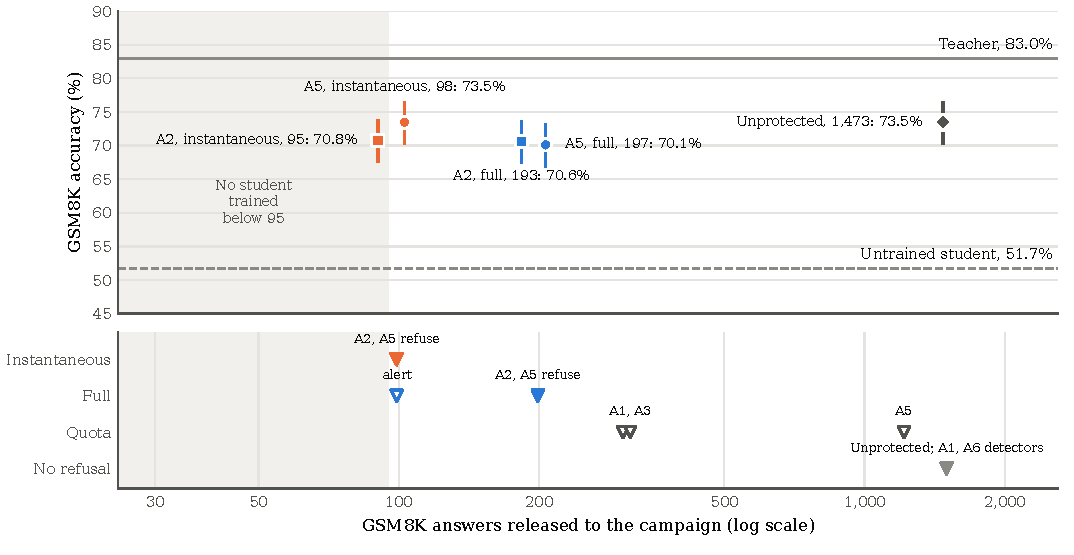
\includegraphics[width=\textwidth]{race.pdf}
\caption{Student accuracy and control interventions on one axis of GSM8K answers. Top: accuracy on 746 held-out problems of five students, each trained on what one v7 arm released, with 95\% Wilson intervals. Students sit at their trainable count, which excludes responses stopped at the output cap. Squares mark A2 (one account, one task at a time) and circles A5 (six accounts, each on one task), offset by 5\% along the axis so that they do not overlap. Table~\ref{tab:campaigns} defines all campaigns. Bottom: GSM8K answers released before each control refused a campaign's math. Filled markers are cuts a student trained on and hollow markers are cuts with no student. The unprotected run sits at 1,500. A replay check before the campaign refused the detector arms of A1 and A6, so they share that marker as the replay's prediction that the detector would never fire. The A2 quota refused before any math and cannot appear on a log axis. The shaded region, below 95 answers, holds no student.}
\label{fig:race}
\end{figure*}

The controls lost the race. Our findings:
\begin{itemize}
	\item \textit{The detector could not see most campaigns.} A replay before each campaign found that the detector never escalated four of the six, while it escalated 10 of 100 held-out legitimate accounts. The simulated users concentrate on one task and topic. A campaign that samples every task looks more ordinary to the detector than those users do.
	\item \textit{When the detector fired, it fired late.} It fired only on accounts that sent a block of math. The first refusal came after 99 math answers under the instantaneous policy and after 199 under the full policy.
	\item \textit{The quota bounded accounts, not campaigns.} It held every account to 1,215 responses. How many math answers that left depended only on the order of each campaign's prompts: none for A2, about 300 for A1 and A3, and 1,215 for A5's math-only account. A campaign split across six accounts, each under the limit, lost nothing.
	\item \textit{What got through was enough.} Students trained on 95 to 197 answers scored 70.1 to 73.5\%. The student trained on all 1,473 scored 73.5\%. No defended student differs from it after Holm correction, and the student trained on 98 answers solved exactly as many problems.
\end{itemize}

We also argue that the late arrival is structural. A detector that scores windows of $W$ requests cannot decide anything about an account before its first window closes. It fires on accounts whose windows are concentrated, so a window that triggers it is mostly one task, and roughly $W$ answers in that task have left by the time it acts. On this bench $W=100$, and 95 answers were already enough.

The evidence has limits that we state up front. It comes from one run, one seed per student, one task and synthetic legitimate users. No student trained on fewer than 95 answers, so we cannot say where the useful supervision starts. We claim only what the panel shows. Every refusal of math we observed, except one quota that ran out before its campaign reached any math, arrived after the released answers had already taught a student most of what the full set taught.

Section~\ref{sec:related} reviews related work. Section~\ref{sec:method} describes the bench and the measurement, and Section~\ref{sec:protocol} the v7 protocol. Section~\ref{sec:timing} reports when each control acted, Section~\ref{sec:students} what the students learned, and Section~\ref{sec:cost} the cost to legitimate users. Section~\ref{sec:discussion} discusses what a control would need to win.

\section{Related work}
\label{sec:related}
\textit{Extraction and distillation.} An attacker queries a victim, collects input-output pairs and trains a surrogate. Task accuracy and fidelity to the victim are different goals~\cite{jagielski2020high}. Krishna et al.\ extracted BERT-based APIs with synthetic queries~\cite{krishna2020thieves}, and Model Leeching reached 75\% exact match on SQuAD for about \$50 in API fees~\cite{birch2023leeching}. Our attacker trains on response-token cross-entropy, which is sequence-level distillation from decoded outputs~\cite{kim2016sequence}, with low-rank adapters~\cite{hu2022lora}. A student can copy a teacher's style without its capability~\cite{gudibande2024false}, so we score students on a benchmark.

\textit{How much supervision a student needs.} Small sets of good answers go a long way. s1 fine-tuned a strong reasoning model on 1,000 curated examples~\cite{muennighoff2025s1}, and LIMO reports strong math reasoning from about 1\% of the data earlier work used~\cite{ye2025limo}. These results concern curated sets and stronger students than ours. They predict, and our panel confirms for one recipe, that an attacker does not need thousands of answers in a task to close most of the gap between a small student and its teacher.

\textit{Per-client detection.} PRADA tracks the distribution of distances between a client's queries, and its authors note that splitting queries across clients defeats it~\cite{juuti2019prada}. Kesarwani et al.\ track feature-space coverage per user~\cite{kesarwani2018warning}, and VarDetect uses latent query distributions~\cite{pal2021stateful}. Liu et al.\ detect extraction in language-model traffic with a kernel two-sample statistic over sentence embeddings and 1,500-query windows~\cite{liu2026detector,mmd2026artifact}. We apply their score per account with 100-request windows. Sun et al.\ show that stateful monitors cannot stop task decomposition across unlinkable identities without denying legitimate traffic~\cite{sun2026decomposition}. Our quota result is the distillation version of that limit.

\textit{Judging defenses by the student.} Libon et al.\ argue that a distillation defense is only broken or unbroken relative to an attacker's query budget, data budget and interface, and show that a larger query budget largely neutralizes antidistillation sampling on GSM8K~\cite{libon2026break}. Allouah et al.\ find that adaptive students recover much more capability than passive evaluation suggests~\cite{allouah2026game}. DistillGuard evaluates output-level defenses on a fixed 10,000-example set and excludes query detection and rate limiting~\cite{jiang2026distillguard}. A lifecycle benchmark scores ten extraction defenses, including MMD, PRADA and SEAT detectors on fixed 50-query batches, and finds that surrogate capability does not always rise with the query budget~\cite{liu2026lifecycle}. None of these measures when an account-level control fires relative to what the student has learned. That is the gap this paper fills.

\textit{Output defenses.} A separate family changes what answers teach. Antidistillation sampling perturbs decoding~\cite{savani2025antidistillation} and trace rewriting turns reasoning into dense formal steps~\cite{ma2026tracerewriting}. Adaptive attackers have recovered much of what such perturbations withhold~\cite{libon2026break,allouah2026game,zhu2026learnability}. The controls we measure leave each answer unchanged and act only on access.

\section{Measuring the race}
\label{sec:method}
\subsection{Gateway and threat model}
One endpoint serves a fixed teacher across four domains, listed in Table~\ref{tab:data}. Each request carries its domain's prompt template and output cap, and the gateway rejects a request that matches no template before any policy decision. Before inference the policy layer sees the prompt, the arrival time and the authenticated account. A campaign controls one or more accounts, collects from every domain, and pools its responses into one training set. The attacker knows how the detector works and sees service actions, but not calibration data or internal scores. Bearer keys give stable identities and put no price on a new account. All accounts in a campaign share one budget of 6,000 HTTP attempts, 1,500 prompts per domain, within 24 hours. Failed requests and proof-of-work submissions spend attempts.

\begin{table}[!t]
\centering\footnotesize
\caption{Domains served by one gateway. Mean tokens are per released response in the unprotected v7 run.}
\label{tab:data}
\begin{tabularx}{\columnwidth}{@{}lYrr@{}}\toprule
Domain & Evaluation & Cap & Mean tokens \\\midrule
AG News~\cite{zhang2015char} & Topic label accuracy & 16 & 2.3 \\
SQuAD 1.1~\cite{rajpurkar2016squad} & Token F1 & 64 & 7.8 \\
GSM8K~\cite{cobbe2021gsm8k} & Numeric exact match & 1,024 & 370 \\
Coding~\cite{ahmad2025opencodeinstruct,liu2023evalplus} & HumanEval+ and MBPP+ pass@1 & 512 & 157 \\\bottomrule
\end{tabularx}
\end{table}

\subsection{Controls}
\label{sec:controls}
The content detector embeds each prompt with \texttt{BAAI/bge-small-en-v1.5}~\cite{xiao2024cpack,bge2023model} and scores each non-overlapping window of 100 consecutive requests from one account against 20 reference windows of pooled benign traffic with the unbiased squared MMD estimator~\cite{gretton2012kernel}. The kernel averages four RBF bandwidths around the median benign distance. Benign calibration windows give $M$ null scores $s_i^{(0)}$, and a window score $s_j$ becomes its upper-tail rank~\cite{phipson2010permutation}
\begin{equation}
p_j=\frac{1+\sum_{i=1}^{M}\I[s_i^{(0)}\geq s_j]}{M+1}.
\end{equation}
A small $p_j$ means the window is rarer than benign windows usually are. The full policy accumulates evidence with a decayed cumulative sum~\cite{page1954cusum},
\begin{equation}
r_{a,j}=\max\{0,\lambda r_{a,j-1}-\log p_{a,j}-\kappa\},\quad r_{a,0}=0,
\label{eq:risk}
\end{equation}
with $\lambda=0.9$ and $\kappa=1$, so a window adds risk only when $p_{a,j}<e^{-1}\approx0.37$. The instantaneous policy keeps no memory and uses $-\log p_{a,j}$ of the current window alone. Thresholds map risk to the levels in Table~\ref{tab:actions}, and an account keeps its highest level until its 24-hour horizon resets.

\begin{table}[!t]
\centering\footnotesize
\caption{Policy levels used in both detector arms.}
\label{tab:actions}
\begin{tabularx}{\columnwidth}{@{}lY@{}}\toprule
Level & Action \\\midrule
L0 & Serve. \\
L1 & Serve and record an alert. \\
L2 & Space admitted requests at least one second apart. \\
L3 & L2, plus a SHA-256 proof of work with 20 leading zero bits. \\
L4 & Refuse until the horizon resets. \\\bottomrule
\end{tabularx}
\end{table}

The quota counts an account's requests in a horizon, serves up to its limit and refuses everything after. It reads no content.

\subsection{Ledger, cuts and students}
The gateway reserves each admission in a release ledger before producing output, and each reservation settles once as released, failed or cancelled. Every released-token count in this paper comes from the ledger. A checkpoint exporter cuts a campaign's ledger at each intervention: the first alert, the first restriction, the first refusal and the end. A student trains on exactly the responses present at its cut, never on a subsample of the final ledger. A response enters training only if the teacher finished it; responses stopped at the output cap are dropped. Figure~\ref{fig:bench} shows the path from request to benchmark.

\begin{figure}[!t]
\centering
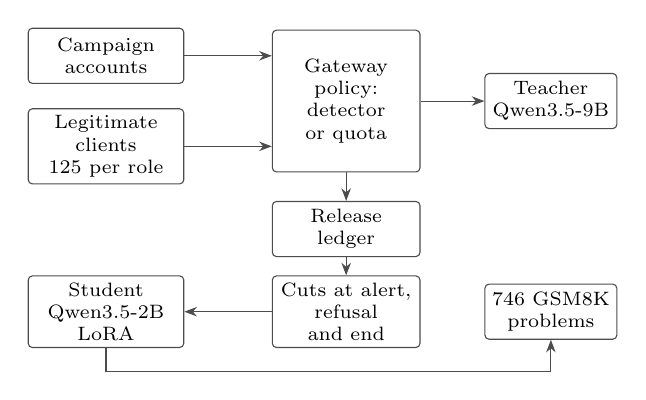
\begin{tikzpicture}[
	font=\scriptsize,
	box/.style={draw=black!70, rounded corners=1.5pt, align=center, inner sep=2.5pt, minimum height=7mm, text width=#1},
	box/.default=18mm,
	arr/.style={-{Stealth[length=1.6mm]}, draw=black!70}
]
\node[box] (atk) at (0, 0) {Campaign\\accounts};
\node[box] (ben) at (0, -1.15) {Legitimate clients\\125 per role};
\node[box=17mm, minimum height=18mm] (gw) at (3.05, -0.575) {Gateway\\policy: detector\\or quota};
\node[box=15mm] (teach) at (5.65, -0.575) {Teacher\\Qwen3.5-9B};
\node[box=17mm] (led) at (3.05, -2.2) {Release ledger};
\node[box=17mm] (cut) at (3.05, -3.25) {Cuts at alert,\\refusal and end};
\node[box] (stu) at (0, -3.25) {Student\\Qwen3.5-2B\\LoRA};
\node[box=15mm] (eval) at (5.65, -3.25) {746 GSM8K\\problems};
\draw[arr] (atk.east) -- (atk.east -| gw.west);
\draw[arr] (ben.east) -- (ben.east -| gw.west);
\draw[arr] (gw) -- (teach);
\draw[arr] (gw) -- (led);
\draw[arr] (led) -- (cut);
\draw[arr] (cut) -- (stu);
\draw[arr] (stu.south) -- ++(0,-3mm) -| (eval.south);
\end{tikzpicture}
\caption{The measurement. Campaign and legitimate traffic share one gateway. The ledger records what the policy let through, and each cut becomes a training set for one student, which is scored on a fixed suite.}
\label{fig:bench}
\end{figure}

\subsection{Indicators}
\label{sec:indicators}
Each model gets its accuracy on the suite with a 95\% Wilson interval~\cite{wilson1927probable}. For a student we also report three ratios built from the untrained student's accuracy $a_0$, the teacher's $a_T$ and the unprotected student's $a_U$.\footnote{The unprotected ledger is the release ledger of campaign A6 under the quota arm. No control fired on that arm, so the ledger holds every one of the 6,000 responses, including all 1,500 GSM8K answers, and we use it as the undefended reference throughout. The unprotected student is the student trained on it.} The gain over the base is $a-a_0$. The share of the base-to-teacher gap closed is $(a-a_0)/(a_T-a_0)$. The share of the unprotected gain kept is $(a-a_0)/(a_U-a_0)$, which is 100\% when withholding cost the student nothing. We compare two models scored on the same items with an exact McNemar test on the items they disagree on~\cite{mcnemar1947note}, Holm-adjusted across all 21 pairs of the seven models~\cite{holm1979simple}, and with a 95\% paired bootstrap interval over items from 10,000 draws~\cite{efron1993bootstrap,koehn2004significance}. For each control we report the GSM8K answers the campaign received before the control refused its math requests.

\section{Protocol}
\label{sec:protocol}
\subsection{Data and users}
We split each domain's pinned source by source group into disjoint roles: development, attacker, benign fitting, score calibration, policy calibration and benign test. We split the attacker role again into an exploratory half for development and a confirmatory half that stays unqueried until a preregistered test. Run v7 used the exploratory half, so it is development evidence. The benign generator creates 125 synthetic accounts per role. About 10\% are generalists that use several domains and the rest are single-domain specialists that send prompts in topic-ordered blocks. Account lengths follow a Pareto distribution with shape 1.5, a 100-request minimum and a 2,000-request cap.

\subsection{Calibration}
Fitting traffic gives the reference windows and kernel bandwidth, score-calibration traffic gives the null, and policy-calibration traffic sets the thresholds so that 10, 5, 2 and 1\% of scored benign horizons reach L1 to L4. We fit the quota to the 1\% target on the same horizons. The v7 null holds 598 window scores, 199 of them from non-overlapping windows, so the smallest attainable rank is $1/599=0.0017$, and 100 scored policy horizons set the thresholds in Table~\ref{tab:cal}. Before any campaign ran, a mixture control scored 50 shuffled windows of pooled benign traffic. All 50 ranked below the median benign account window, with a median rank of 0.970. Under this score, a window that looks like the average of all users looks more ordinary than almost any single user.

\begin{table}[!t]
\centering\footnotesize
\caption{The v7 calibration on 100 scored policy horizons. Upper bounds are Clopper-Pearson 95\%~\cite{clopper1934limits}.}
\label{tab:cal}
\begin{tabularx}{\columnwidth}{@{}Ycccc@{}}\toprule
 & L1 & L2 & L3 & L4 \\\midrule
Target rate & 0.10 & 0.05 & 0.02 & 0.01 \\
Upper bound at target & 0.164 & 0.102 & 0.062 & 0.047 \\
Full thresholds & 0.38 & 1.50 & 2.76 & 4.01 \\
Instantaneous thresholds & 1.38 & 2.24 & 3.06 & 3.50 \\
Quota, requests per horizon & & & & 1,215 \\\bottomrule
\end{tabularx}
\end{table}

\subsection{Campaigns}
Table~\ref{tab:campaigns} lists the eight campaign designs in the harness and what each tests. v7 ran six of them. A4 repeats A1 at a lower declared request rate, and A8 picks its next prompts from what it observes during collection. Both are implemented and neither was run in v7, so the numbering skips them. A1, A2, A5 and A6 send the same prompts and differ only in order and account ownership. Each campaign runs against three arms: the full policy, the instantaneous policy and the quota. Every arm gets a fresh gateway, fresh credentials and its own state. Before a detector arm sends a request, a detectability check replays the frozen campaign offline through the served calibration together with the 125 held-out benign accounts. The arm runs only if the campaign's highest level in replay is above L0 and fewer than 10\% of the benign horizons reach that level. Otherwise the arm sends nothing and the runner records it as refused. A refused arm is still a detector result, because the replay predicts that the live arm would release everything.

\begin{table}[!t]
\centering\footnotesize
\caption{Collection campaigns. A4 and A8 are implemented and were not run in v7.}
\label{tab:campaigns}
\begin{tabularx}{\columnwidth}{@{}lYY@{}}\toprule
ID & Accounts and order & What it tests \\\midrule
A1 & One account; domains interleaved. & Broad extraction, the baseline. \\
A2 & One account; one block per domain, AG News first, GSM8K second. & Collecting one task at a time. \\
A3 & One account; half the budget spent on in-distribution cover traffic. & Cover traffic that dilutes the detector's score. \\
A4 & A1 at a lower declared request rate. & Not run. \\
A5 & Six accounts, one domain each: two AG News, two coding, one SQuAD, one GSM8K. & Splitting accounts by task. \\
A6 & Six accounts; A1's prompts split across them by a seeded permutation. & Splitting accounts at random. \\
A7 & One account; prompts from separately pinned corpora, MathQA for math. & Prompts from sources other than the other campaigns'. \\
A8 & Picks prompts from feedback observed during collection. & Not run. \\\bottomrule
\end{tabularx}
\end{table}

\subsection{Teacher, students and suite}
The teacher is \texttt{Qwen3.5-9B}~\cite{qwen2026qwen35} quantized to Q4\_K\_M, served by llama.cpp~\cite{llamacpp} on one laptop RTX~4060 in non-thinking mode at temperature 0. Every student is a LoRA adapter on \texttt{Qwen3.5-2B-Base} with rank 16, $\alpha=32$ and dropout 0.05 on all linear layers, trained for three epochs at learning rate $10^{-4}$ with an effective batch of 16, a 2,048-token limit, bf16 weights~\cite{hu2022lora,loshchilov2019adamw} and seed 42. We trained five students, one on the end ledger of each detector arm that released math (A2 and A5 under both policies) and one on the unprotected ledger, which holds all 1,500 GSM8K answers. In A2 and A5 no math arrived after the refusal, so each end ledger equals its refusal ledger. We trained no quota students.

We score the students and the base with greedy decoding and a 512-token limit on a frozen 746-problem GSM8K development suite, and the teacher through the same API the campaigns used. Before training any student we set 65\% as the accuracy threshold for a useful student. On 746 items a binary accuracy has a 95\% half-width of about 3.6 points near 50\%, and a paired comparison with 20\% discordant items resolves about 4.6 points at 80\% power~\cite{connor1987paired,card2020power}.

\section{When the controls act}
\label{sec:timing}
Table~\ref{tab:timing} gives, for every campaign and arm, how many GSM8K answers the campaign had received when the control refused its math. The rest of this section explains the pattern.

\begin{table}[!t]
\centering\footnotesize
\caption{GSM8K answers released to each v7 campaign before the control refused its math, from the release ledger. ``Never'' under a detector means the replay check refused the arm because the campaign never escalated, so the arm would release its whole budget. A7's math is MathQA.}
\label{tab:timing}
\begin{tabularx}{\columnwidth}{@{}lYYY@{}}\toprule
Attack & Full & Instantaneous & Quota \\\midrule
A1 & never & never & 303 \\
A2 & alert 99, refuse 199 & refuse 99 & 0 \\
A3 & never & never & 314 \\
A5 & alert 99, refuse 199 & refuse 99 & 1,215 \\
A6 & never & never & never, 1,500 (unprotected) \\
A7 & never & never & 303 MathQA \\\bottomrule
\end{tabularx}
\end{table}

\subsection{The detector cannot see broad campaigns}
The detectability check refused both detector arms for A1, A3, A6 and A7. In replay each campaign stayed at L0 under both policies, while the same replay escalated 10 of the 100 scored held-out benign horizons under each policy. Under the full policy 4 of them reached refusal, above the 1\% target and inside its 4.7\% upper bound. The earlier run v5, on a different teacher build, refused the same eight arms.

The mixture control explains why. Legitimate users in this generator concentrate on one task and topic, so their windows sit far from the pooled reference. A campaign that samples every task sits close to it. The score ends up measuring topic concentration, and a broad campaign is less concentrated than the users it hides among. An audit of the earlier v3 run found that sorting the same 6,000 prompts by topic within each domain moved every window back into the benign bulk, under upper-tail, lower-tail and two-sided variants alike~\cite{trace2026artifact}.

\subsection{When the detector fires, it fires one window late}
The detector escalated A2 and A5, and in both it escalated on math. Figure~\ref{fig:ranks} shows A5's window ranks. The GSM8K account's two windows ranked 0.015 and 0.030. Every window from the other five accounts ranked above 0.42 and added no risk, so those accounts stayed at L0 and received 4,494 responses, including 1,494 coding answers.

\begin{figure}[!t]
\centering
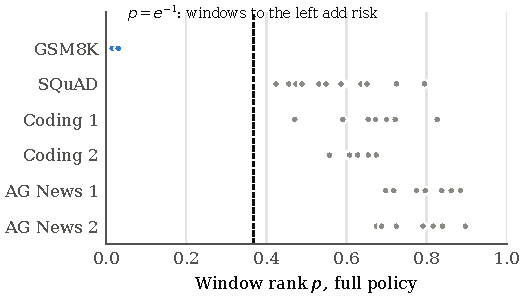
\includegraphics[width=\columnwidth]{a5-ranks.pdf}
\caption{Window ranks of A5's six accounts under the full policy. Only windows left of the dashed line add risk. The GSM8K account reached L4 and the other five stayed at L0.}
\label{fig:ranks}
\end{figure}

The timing follows from the window. A rank exists only once a 100-request window closes, so the first possible decision about the GSM8K account came at its 100th math request. Under the full policy the first window's rank of 0.015 gave a risk of 3.20 by Eq.~\eqref{eq:risk}. That cleared the L3 threshold but not the L4 threshold of 4.01, which a single window reaches only with a rank below about 0.007. Under the instantaneous policy the same window scored $-\log 0.015=4.20$, above its L4 threshold of 3.50. Under the full policy the account received a proof-of-work challenge, which cost the campaign 100 attempts, and was refused at its 200th math request after 199 answers. The instantaneous policy refused at the 100th, after 99 answers. A2 behaved the same way inside its GSM8K block, after 1,500 AG News prompts that the detector ignored.

\subsection{The quota bounds accounts, not campaigns}
The quota fired where it was set. It held each account to at most 1,215 responses and refused every request from attempt 1,216. How much math that left depended only on the order of each campaign's prompts. A1 and A3 interleave domains and kept 303 and 314 math answers. A2 sends AG News first, so its quota ran out on one-word labels and it kept no math at all. That is the only refusal on this bench that withheld all math, and it came from the order of the campaign, not from anything the control noticed. Against account splitting the quota did what its definition implies. A5's GSM8K account kept 1,215 math answers. A6 spread its prompts over six accounts that each stayed under the limit and received all 6,000 responses. That ledger is the unprotected run.

\subsection{Tokens tell a different story}
Measured in tokens, the detector looked effective against A5. GSM8K answers averaged 370 tokens and AG News answers 2.3, so refusing one math account removed most of the campaign's tokens. Figure~\ref{fig:tokens} shows the breakdown. Under the full policy A5 received 321,831 tokens, 40\% of the 806,570 the unprotected run received, and 71,142 GSM8K tokens, 12.8\% of 555,498. A provider that scores its controls by tokens withheld would count this as a success. Section~\ref{sec:students} asks whether the student agrees.

\begin{figure}[!t]
\centering
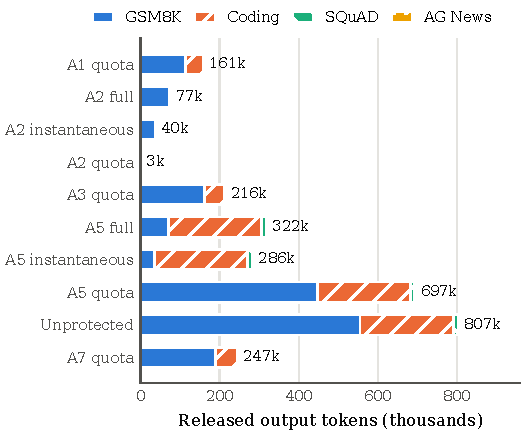
\includegraphics[width=\columnwidth]{tokens.pdf}
\caption{Released output tokens by domain for every v7 arm that ran, from the release ledger. SQuAD and AG News responses are too short to show at this scale.}
\label{fig:tokens}
\end{figure}

\section{What the students learned}
\label{sec:students}
Table~\ref{tab:students} reports the panel. Every student learned. The weakest gained 18.4 points over the untrained student and the strongest 21.7, and all five cleared the 65\% target set before training. The four defended students trained on 6.4 to 13.4\% of the unprotected run's answers and closed 59 to 70\% of the gap between the base and the teacher. The unprotected student closed 70\%.

\begin{table*}[!t]
\centering\footnotesize
\caption{The v7 GSM8K student panel on 746 development problems. Trainable answers exclude responses stopped at the output cap. Ratios are defined in Section~\ref{sec:indicators}. The last two columns compare each student with the unprotected student: a paired item-bootstrap 95\% interval and the exact McNemar $p$, with the Holm-adjusted value across all 21 model pairs in parentheses. Optimizer steps follow from the recipe as $3\lceil n/16\rceil$. The teacher row is the pass used for every comparison; two repeat passes scored 620 and 626.}
\label{tab:students}
\setlength{\tabcolsep}{3pt}
\begin{tabular*}{\textwidth}{@{\extracolsep{\fill}}lrrcrrrrcc@{}}\toprule
Model & Answers & Steps & Accuracy, \% [Wilson 95\%] & Correct & Gain, pts & Gap closed & Gain kept & Minus unprotected, pts & $p$ (Holm) \\\midrule
Untrained student & 0 & 0 & 51.7 [48.2, 55.3] & 386 & & & & & \\
A2, instantaneous & 95 & 18 & 70.8 [67.4, 73.9] & 528 & 19.0 & 61\% & 88\% & $-2.7$ [$-5.9$, $+0.5$] & 0.11 (0.55) \\
A5, instantaneous & 98 & 21 & 73.5 [70.2, 76.5] & 548 & 21.7 & 70\% & 100\% & $0.0$ [$-3.1$, $+2.9$] & 1.00 (1.00) \\
A2, full & 193 & 39 & 70.6 [67.3, 73.8] & 527 & 18.9 & 61\% & 87\% & $-2.8$ [$-5.9$, $+0.1$] & 0.082 (0.49) \\
A5, full & 197 & 39 & 70.1 [66.7, 73.3] & 523 & 18.4 & 59\% & 85\% & $-3.4$ [$-6.3$, $-0.4$] & 0.034 (0.31) \\
Unprotected & 1,473 & 279 & 73.5 [70.2, 76.5] & 548 & 21.7 & 70\% & 100\% & & \\
Teacher & & & 83.0 [80.1, 85.5] & 619 & 31.2 & & & & \\\bottomrule
\end{tabular*}
\end{table*}

Figure~\ref{fig:supervision} sets the two ratios that matter side by side. The detector withheld 87 to 94\% of the math answers a student could train on. The students kept 85 to 100\% of what the full set taught. Withholding was large in supervision and small in capability.

\begin{figure}[!t]
\centering
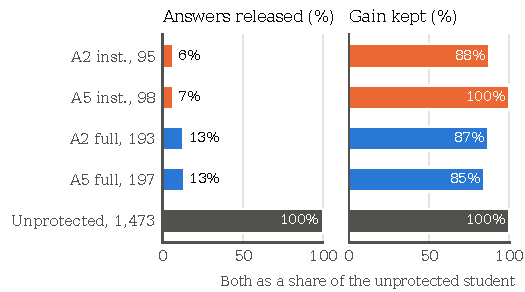
\includegraphics[width=\columnwidth]{supervision.pdf}
\caption{Left: GSM8K answers each defended student trained on, as a share of the unprotected run's 1,473. Right: each student's gain over the untrained student, as a share of the unprotected student's 21.7-point gain.}
\label{fig:supervision}
\end{figure}

\subsection{Differences between students}
Figure~\ref{fig:paired} shows each defended student minus the unprotected one. The point estimates run from $-3.4$ to 0.0 points. Only A5 under the full policy has a raw McNemar $p$ below 0.05, 0.034 on 52 against 77 discordant items, and Holm adjustment across the panel moves it to 0.31. The 98-answer student and the 1,473-answer student solved exactly 548 problems each and disagreed on 130, split 65 and 65.

\begin{figure}[!t]
\centering
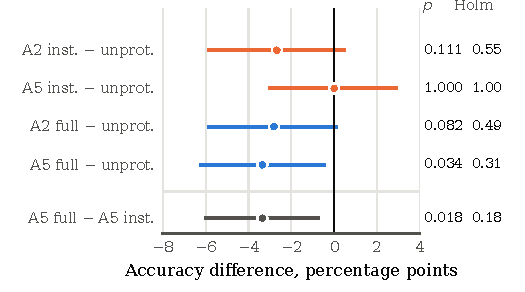
\includegraphics[width=\columnwidth]{paired.pdf}
\caption{Paired accuracy differences on the 746 problems with 95\% item-bootstrap intervals. The right columns give the exact McNemar $p$ and its Holm adjustment across all 21 model pairs. The bottom row compares two defended students from the same campaign.}
\label{fig:paired}
\end{figure}

The panel also shows how far one-seed students move for reasons other than data size. A5 under the instantaneous policy trained on 98 answers and beat A5 under the full policy, trained on 197, by 3.4 points (raw $p=0.018$, Holm 0.18). The student with half the data did better, by the same margin that separates the full-policy A5 student from the unprotected one. With one training seed per student, a three-point difference is within the spread this panel shows between students that differ in something other than data size. We read the 3.4-point gap between A5 under the full policy and the unprotected student in that light.

The recipe adds a second confound. It trains for three epochs at any size, so the unprotected student took 279 optimizer steps and the instantaneous A5 student 21. More data came with more training, yet the student with a thirteenth of the steps tied the one with all of them. If extra steps help at all here, they did not show.

\subsection{Inference is not the noise}
We re-ran inference three times for every model on the same 746 problems. All five students and the base produced byte-identical outputs on every pass, so their scores carry no decoding noise. The teacher, served through llama.cpp, scored 619, 620 and 626, a spread of 0.9 points. We use the 619 pass throughout. Resampling by normalized question family instead of by item widens the unprotected student's interval only to 70.1 to 76.7\%.

\section{Cost to legitimate users}
\label{sec:cost}
Table~\ref{tab:cost} gives the benign cost two ways. The offline replay asks how many held-out accounts a control escalates. Under either detector policy it was 10 of 100. Under the full policy 4 reached refusal. Under the quota one held-out account of 125 sends more than 1,215 requests. It sends 1,832 and loses 617, about 2.6\% of all benign-test requests.

\begin{table}[!t]
\centering\footnotesize
\caption{Benign cost in v7. Replay uses 100 scored held-out benign horizons for the detectors and 125 held-out accounts for the quota. The live pass sent the 24,047-request benign-test schedule through each arm.}
\label{tab:cost}
\begin{tabularx}{\columnwidth}{@{}Yrrr@{}}\toprule
 & Full & Inst. & Quota \\\midrule
Replay: accounts escalated & 10 & 10 & 1 \\
Replay: reaching L1, L2, L3 & 5, 1, 0 & 5, 0, 3 & \\
Replay: refused & 4 & 2 & 1 \\
Live: benign requests refused & 464 & 0 & 0 \\
Live: served-only quality & 0.822 & 0.834 & 0.835 \\
Live: completion & 9.3\% & 11.3\% & 11.8\% \\\bottomrule
\end{tabularx}
\end{table}

The live pass measures something else, and on this hardware mostly the teacher. With a 120-second client deadline the laptop teacher completed only 9 to 12\% of requests under every arm, and about 21,300 timed out each time. Completion therefore measures teacher capacity, not policy cost. The comparable live numbers are refusals and the quality of what was served. The full policy refused 464 benign requests and the other two arms none. The quota refused nobody live because most requests timed out before admission. The utility pass ran after each campaign on separate accounts, so no run has measured a real mixture of attack and benign traffic.

Set against Section~\ref{sec:students}, these costs buy little. The full policy refused 4 of 100 held-out legitimate accounts in replay and 464 live requests, and its refusals of A2 and A5 came after students on the released answers already scored at or near the unprotected level.

\section{Discussion}
\label{sec:discussion}
\subsection{Why a window detector arrives late}
The detector on this bench decides only when a window closes. Call the window length $W$ and suppose an account sends a fraction $c$ of its requests in one task. The earliest decision about the account comes after $W$ requests, of which about $cW$ are in that task. The detector fires on accounts that look concentrated, which means $c$ near 1, because concentration is what moves the score away from the pooled reference. So when it fires on a task, roughly $W$ answers in that task have already left. Campaigns with small $c$ would be caught earlier in task terms if they were caught at all, but those are exactly the campaigns that look like the average user and are never caught. Memory delayed the full policy further. It needed two windows and released 199 answers, and the instantaneous policy needed one window and released 99.

On this bench $W=100$ and $c=1$ for A2's math block and A5's math account, and students trained on 95 to 98 answers already reached 70.8 and 73.5\%. To have withheld the supervision that produced those students, the detector would have had to refuse at well under 100 answers. We have no student below 95, so we cannot say how far under.

Shrinking $W$ is the obvious response, and it has a price. The score of a smaller window is noisier, so its null spreads out and a legitimate specialist's block of 20 math prompts looks like an attacker's. With 100-request windows the replay already escalated 10 of 100 held-out legitimate accounts and refused 4. We did not measure smaller windows, and doing so is the clearest next experiment for the detector.

\subsection{Tokens are the wrong score}
By released tokens the full policy cut A5 to 40\% of the unprotected run and its GSM8K tokens to 12.8\%. By student accuracy it cut nothing that survived correction. Token and request counts are what a gateway sees, so they are the natural numbers to report. They are also the numbers that most overstate an account-level control. A control that withholds 87\% of a task's answers after the first 199 can look strong on every dashboard and still leave the attacker with a student it can use. We think defenses aimed at distillation should report student accuracy at the cut where they intervened, next to what they cost legitimate users.

\subsection{What could act in time}
The quota bounds what one account receives, and the ledger confirmed the bound to the request. It says nothing about a campaign, because a campaign can add accounts. A6 did and lost nothing. This repeats, for distillation, the limit Sun et al.\ prove for decomposition attacks across unlinkable identities~\cite{sun2026decomposition}. Controls that act on account creation and coordination, such as linking accounts through payment or infrastructure and verifying identity~\cite{anthropic2026detecting,openai2026disrupting}, aim at the weakness the quota leaves. A per-account budget counted in output tokens rather than requests would at least have treated a math account and a news account differently. Every one of these still has to fire before about a hundred answers in a task to beat the students in our panel, and none has a measured false-positive rate on this bench.

Output defenses take the other route and change what each answer teaches~\cite{savani2025antidistillation,ma2026tracerewriting}. They do not depend on timing, but adaptive attackers have recovered much of what they withhold~\cite{libon2026break,allouah2026game,zhu2026learnability}. Our measurement applies to them unchanged. Cut the ledger where they act and train on what went out.

\section{Limitations}
\label{sec:limits}
The student evidence is one task, one recipe, one training seed per student and five students. The paired tests resample problems, not training runs, so they cannot see seed variance, and the panel itself suggests that variance is about three points. The recipe ties optimizer steps to data size. No student trained on fewer than 95 answers, so where useful supervision begins is unmeasured. The legitimate users are synthetic, and their topic concentration drives the detector result. A provider whose users are mostly math tutors would see a different picture. All campaigns use one seed and the exploratory half of the attacker data. The utility pass ran after each campaign on a teacher that could serve only about a tenth of its requests within the deadline. The teacher's 83.0\% scores 96 answers that were cut at the 512-token limit as they stand, so it may understate the teacher. Bearer keys stand in for identity, and nothing prices a new account. Coding answers, which no detector arm withheld, have no student.

\section{What would sharpen the result}
\label{sec:next}
All of the following reuse the v7 ledgers and need no new campaign. A learning curve on random subsets of the unprotected run's GSM8K answers, at 10, 25, 50, 100, 200, 400 and 800 with several seeds each, would measure where the useful supervision starts and turn the shaded region of Figure~\ref{fig:race} into data. Two more seeds for each existing student would put an interval on training variance. Students at matched optimizer steps would separate data from training length. A coding student would test a second task, one where no detector arm withheld anything. A detector with smaller windows, calibrated on the same benign roles, would show what an earlier refusal costs legitimate users. Finally, a campaign on the sealed confirmatory half would turn this development evidence into a test.

\section{Conclusion}
An account-level control can only protect a teacher if it acts before the attacker holds enough supervision. We measured both sides of that race on one bench. On GSM8K, every refusal that withheld math came after at least 99 answers, except a quota that ran out on news labels first, and students trained on 95 to 197 answers kept 85 to 100\% of what 1,473 answers taught. The detector never saw four of six campaigns and the quota never saw a split one. The controls rationed tokens and left the student's accuracy where it would have been without them. The bench, the run records and the per-item student scores are public~\cite{trace2026artifact}.

\bibliographystyle{IEEEtran}
\bibliography{references}
\end{document}
